\chapter{Task 01: Ising Model}
\section{Task Description}
The aim of this task is to simulate the Ising dynamics on complex networks.
\section{Mathematical model}
The ferromagnetic Ising model on a network of $N$ nodes and adiacency matrix $A$ is described in its most general form by the hamiltonian:
\begin{equation*}
    \mathcal{H}\{\mathbf{s}\} = - \sum_{i < j}\, J_{i,j}\,s_i\cdot s_j - \sum_{i}\, h_i\,s_i
\end{equation*}
where $\mathbf{s} = (s_1, \cdots s_N)$, $s_i = \pm 1$ is the spin configuration of the nodes, the couplings $J_{i,\,j}$ describe the pairwise spin interactions and $h_i$ is a site-dependent external field.
In the following, it will be always assumed $J_{i,\,j} \equiv 1\cdot A_{i,\,j}$ (only nearest neighbours interactions of homogeneous strength) and $h_i \equiv h$ (homogeneous external field), so that the hamiltonian becomes
\begin{equation}
        \mathcal{H}(\mathbf{s}) = - \sum_{i < j}\, A_{i,j}\,s_i\cdot s_j - h\cdot \sum_{i}\,s_i
\end{equation}
The network is surrounded by a heat bath at temperature $T = \frac{1}{\beta} $ ($k_B \equiv 1$). The partition function $Z$ and the free energy $F$ are given by:
\begin{equation*}
    Z\left(T, \{A_{i,\,j}\}, h, N\right) = \sum_{\mathbf{s}}\, e^{-\beta\, \mathcal{H}(\mathbf{s})} \quad F = -\frac{1}{\beta}\, \text{ln}[Z]
\end{equation*}
The most relevant thermodynamic quantities are the internal energy $E$, the magnetization $M$, the specific heat $C$ and the magnetic susceptibility $\chi$:

\begin{align*}
E &= \mathbbm{E}[\mathcal{H}(\mathbf{s})], &
C &= \left( \frac{\partial E}{\partial T} \right)_{h} \equiv \frac{\mathbbm{E}[E^2] - \mathbbm{E}[E]^2}{T^2} \\
M &= \mathbbm{E}\left[\sum_{i} s_i \right] \equiv \left( \frac{\partial F}{\partial h} \right)_{\beta}, &
\chi &= \left( \frac{\partial M}{\partial h} \right)_{T} = -\left( \frac{\partial^2 F}{\partial^2 h} \right)_{T} \equiv \frac{\mathbbm{E}[M^2] - \mathbbm{E}[M]^2}{T^2}
\end{align*}


By means of a mean field approximation, it is possible to show that the existence of a disordered phase depends on the moments $\<k^n\>$ of the degree distribution. Specifically, a homogeneous mean field approximation yields the critical temperature
\begin{equation} \label{eq:hom_mean_field}
    T_C^{\text{hom. MF}} =\,\left\langle k \right \rangle
\end{equation}
(see appendix [App \ref{app:mean_field}] for complete derivation), while the more accurate heterogeneous (or degree-based) mean field approximation yields:
\begin{equation} \label{eq:het_mean_field}
    T_C^{\text{het. MF}} =\,\frac{\left\langle k^2 \right \rangle}{\left\langle k \right \rangle}
\end{equation}
In particular, the latter formula is derived under the assumption that the network is uncorrelated, that is, the nearest neighbour degree distribution is the same as in the configuration model $P_{n.n.} (k)=\frac{k\cdot P(k)}{<k>}$.
The exact value of the critical temperature, as well as the critical exponents, are found via the replica approach \cite{analytical_ising}. \\ 
The order parameter of the transition is the average magnetization per site, $s$:
$$
s := \frac{M}{N} = \mathbbm{E}\left[\frac{\sum_{i}\,s_i}{N}\right]
$$
which is zero in the disordered phase ($T>T_C$), non-zero in the ferromagnetic  phase $(T<T_C)$ and monotonically decreasing with temperature. Also, the energy $E(T)$ is expected to have an inflection point at $T=T_C$, and the response function $C$ and $\chi$ are both supposed to peak at $T=T_C$.

\section{Numerical Simulations}
For simulations, I chose to focus on scale free networks $P(k) \sim k^{-\gamma}$, in particular the Barabasi - Albert (BA) network of parameters $N,\, m$ where N is the number of nodes and $m$ is the number of links attacched for each new node. This choice was motivated by the fact that article \cite{numeric_ising} could be used for comparison. The degree distribution for such a network is asymptotically given by $P(k) \sim k^{-3}$. Since one can only deal with finite size networks, finite size effects must be taken into account in the mean field formulas $\ref{eq:hom_mean_field}$ and $\ref{eq:het_mean_field}$.
The finite size of the network implies the existence of a cutoff degree $k_{max}(N)$, so the right estimation of the moment $\left\langle k^n \right \rangle$ is given by
\begin{equation*}
    <k^n> = \sum_{k=m}^{k_{max}(N)}\, k^n\,P(k)
\end{equation*}
where the cutoff $k_{max}(N)$ is defined such that the probability of having a node of degree $k>k$ in a network of size $N$ is less than one. With an elementary calculation one can verify that $k_{max}(N)= m\cdot N^{\frac{1}{\gamma -1}}$, which reduces to $k_{max} = m\cdot \sqrt{N}$ for a BA network.
The average degree is left unchanged by the finite size correction:  $<k> = 2m$, whereas the second moment changes to $<k^2> \simeq m^2\,\text{ln}(N)$ \cite{analytical_ising}. Hence, the critical temperatures given by the mean field formulas are:
\begin{equation}
    T_C^{\text{hom. MF}} = 2m, \quad \quad T_C^{\text{het. MF}} \simeq \frac{m}{2}\,\text{ln}(N)
\end{equation}
The heterogeneous mean field approximation predicts a logaritmic increase of the temperature with the network size, which means that in the thermodynamic limit ($N\rightarrow +\infty$) the network is expected to be ferromagnetic at all temperatures: this agrees with the exact replica calculation $\cite{analytical_ising}$. The homogeneous mean field is too drastic and fails to predict this behaviour. Also, the critical temperature is expected to increase with the average degree, which indicates that adding more connections between the nodes helps in mantaining long-range order. \\
For my simulations, I chose to investigate both the finite size effect and the linear dependence on $m$ predicted by the heterogeneous mean field formula.




\newpage
\subsection*{Appendix}
\addcontentsline{toc}{section}{Appendix}
\subsection*{Mean field calculations} \label{app:mean_field}
{\small
The mean field approximation consists in negletting the pairwise spin correlations:
\begin{equation*}
    \text{corr}(s_i,\,s_j) = (s_i - \left\langle s_i \right \rangle)\cdot (s_j - \left\langle s_j \right \rangle)\simeq 0
\end{equation*}
Moreover, the homogeneous mean field supposes that the average magnetization on each node is the same for all nodes $\left\langle s_i\right\rangle \equiv \left \langle s \right \rangle$, while the heterogeneous mean field makes the weaker assumption that the average magnetization on a node depends at most on the node's degree: $\left \langle s_i\right \rangle \equiv \left\langle s_{k_i}\right\rangle$. 
Let's consider the homogeneous mean field for simplicity. We start from the hamiltonian $H\{\mathbf{s}\} = -\frac{1}{2}\, \sum_{i,\,j}\,A_{i,\,j}\,s_i\cdot s_j - h\cdot\sum_{i}\,s_i$. We can write the identity 
\begin{align*}
    s_i\cdot s_j &= [s_i - \left\langle s \right \rangle + \left\langle s \right \rangle]\cdot [s_j - \left\langle s \right \rangle + \left\langle s \right \rangle] \\
    &= (s_i - \left\langle s \right \rangle)\cdot (s_j-\left\langle s \right \rangle) + (s_i + s_j) \left\langle s \right \rangle - \left\langle s \right \rangle^2 \simeq (s_i + s_j) \left\langle s \right \rangle - \left\langle s \right \rangle^2
\end{align*} where the latter is obtained disregarding the correlation term. With this substitution, the hamiltonian becomes 
\begin{equation*}
    H \simeq\frac{1}{2}\,\left\langle s \right \rangle^2\,N\,\left\langle k \right \rangle - \sum_i\,s_i\cdot (\left\langle k \right \rangle\left\langle s \right \rangle + h)=: H^{MF}(\mathbf{s})
\end{equation*}
This expression can be now used to compute the partition function:
\begin{align*}
    Z^{MF} &= \sum_{\mathbf{s}}\, e^{-\beta H^{MF}(\mathbf{s})} = e^{-\beta \frac{N \left\langle k \right \rangle\left\langle s \right \rangle^2}{2}}\, \sum_{\mathbf{s}}\, e^{\beta\left[(<k><s> + h)\sum_l\,s_l\right]} \\
    &= e^{-\beta \frac{N <k><s>^2}{2}}\, \prod_{i=1}^{N}\, \left[ \sum_{s = \pm 1}\, e^{\beta(<k>+h)\,s_i} \right] \\
    &= e^{-\beta \frac{N \left\langle k \right \rangle\left\langle s \right \rangle^2}{2}}\,\left[2\,\text{cosh}\left[\beta(\left\langle s \right \rangle\left\langle k \right \rangle+h)\right]\right]^N
\end{align*}
The free energy per node is then:
\begin{equation*}
   f^{MF}= \frac{F^{MF}}{N} = - \frac{1}{N\beta}\text{ln}[Z^{MF}] = \frac{1}{2}\left\langle k \right \rangle\left\langle s \right \rangle^2 -\frac{1}{\beta}\text{ln}\left[2\,\text{cosh}[\beta(\left\langle s \right \rangle\,\left\langle k \right \rangle+h)]\right]
\end{equation*}
\begin{minipage}{0.55\textwidth}
The average magnetization per site is given by
\begin{equation*}
    <s> = -\left(\frac{\partial f^{MF}}{\partial h}\right)_\beta \equiv \text{tanh}[\beta(<s><k>+h)]
\end{equation*}
When the external field is off, $<s>$ is the solution of the implicit equation $<s> = \text{tanh}[\beta\,<s>\,<k>]$, which is the interesection of $y = <s>$ and $y = \text{tanh}[\beta\,<s>\,<k>]$.
For $\beta < \beta_C = \frac{1}{<k>}$, there are no intersection points (the system is paramagnetic) for $\beta > \beta_C$ there are two simmetric intersections (the system is ferromagnetic). \\
In the heterogeneous mean field, very similiar calculations \cite{analytical_ising} lead instead to the equations:
\begin{align*}
    <u> &= \sum_{k}\, \frac{k P(k)}{<k>}\,\text{tanh}[\beta ( k <u>)] \\ <s> &= \sum_k \, P(k)\,\text{tanh}[\beta ( k <u>)] 
\end{align*}
\end{minipage}
\hfill
\begin{minipage}{0.38\textwidth}
\centering
    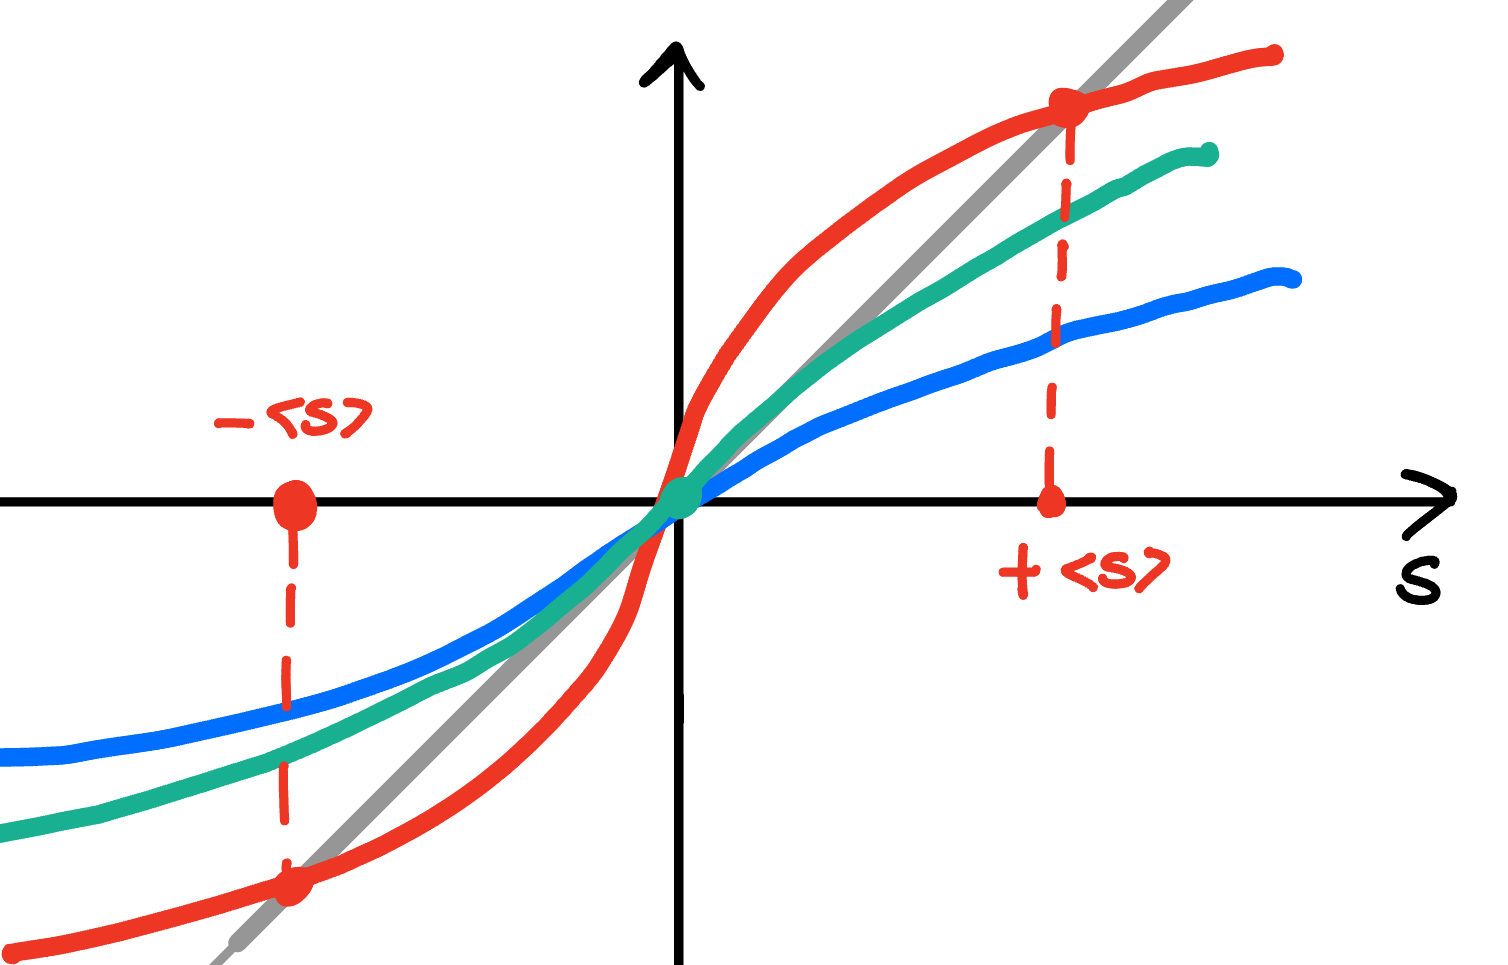
\includegraphics[width = \textwidth]{latex_source/images/ising/IMG_56FE6CFC861B-1.jpeg}
    \captionof{figure}{\small Grey line is $y=s$, coloured lines are $y = \text{tanh}(\beta <k> s)$, respectibely for $\beta\,<k> > 1$ (red, ferromagnetic state), $\beta\,<k> > 1$ (green, critical point) and $\beta\,<k> < 1$ (blue, paramagnetic state).}
\end{minipage}
\subsection*{Preliminary simulation on a 2D lattice}
{\small
To check the correctness of my code, I first tested it on a 2D lattice. This way, I could look by eye if the code behaved as expected and get an estimate of the computation time required before moving to more complicated simulations. 
In 2D, an infinite regular spin lattice exibits a second order phase transition at the critical
temperature 
\begin{equation}
T_C = \frac{2\,J}{k_B\,\log{1 + \sqrt{2}}} \simeq 2.26
  \end{equation}  
    \label{eq:onsager}
(A finite lattice of linear dimention $N$ exibits finite size effect, so the estimated critical temperature is slightly different from the Onsager formula.)
For my simulation, I considered a lattice of $N = 20 \cdot 20 = 400$ nodes. I first simulated the dynamics at fixed temperature, to get an estimate of the number of steps required for the system to equilibrate. I found that $\simeq 500$ steps where sufficent for a lattice of this size [Fig \ref{fig:2d_relaxation}]. Then I simulated Ising over a broad range of temperatures around the expected critical temperature and computed the energy, magnetization, heat capacity and magnetic susceptibility [Fig: \ref{fig:2d_scaling}].
}
\begin{figure}[H]
    \centering
    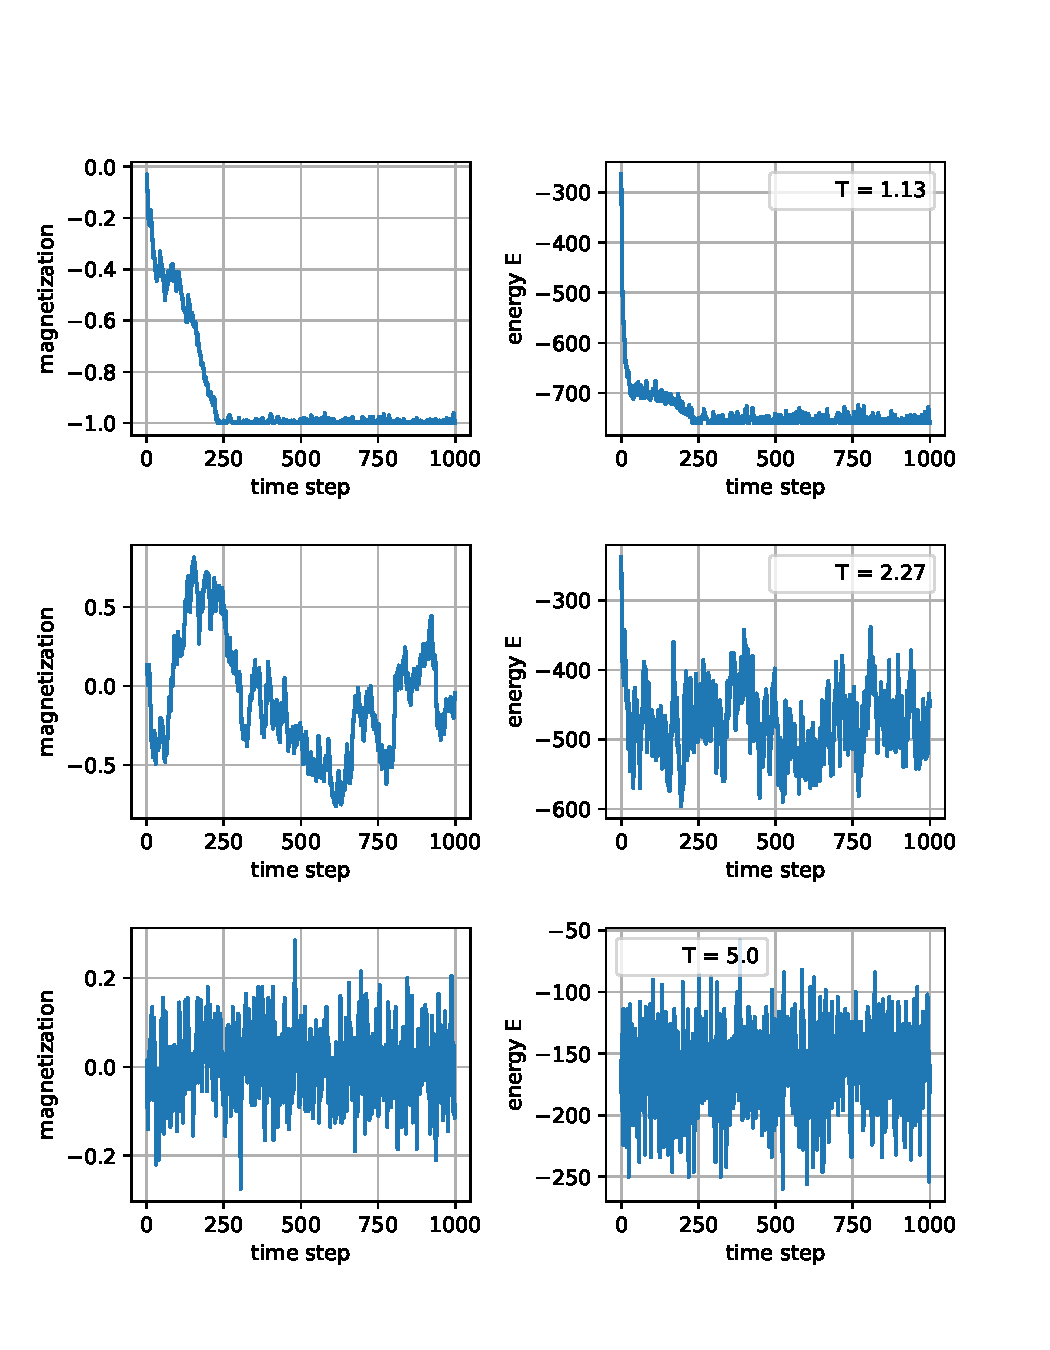
\includegraphics[width=0.6\linewidth]{latex_source/images/ising/2d_relaxation.pdf}
    \caption{{\small Time evolution of the magnetization and energy, respectively below, at and above the critical temperature $T_C \simeq 2.26$. From the top figure ($T = 1.13 < T_C$ one can see that approximately $\sim\,250$ Metropolis steps are enough for the sistem to equilibrate.}}
    \label{fig:2d_relaxation}
\end{figure}

\begin{figure}[H]
    \centering
    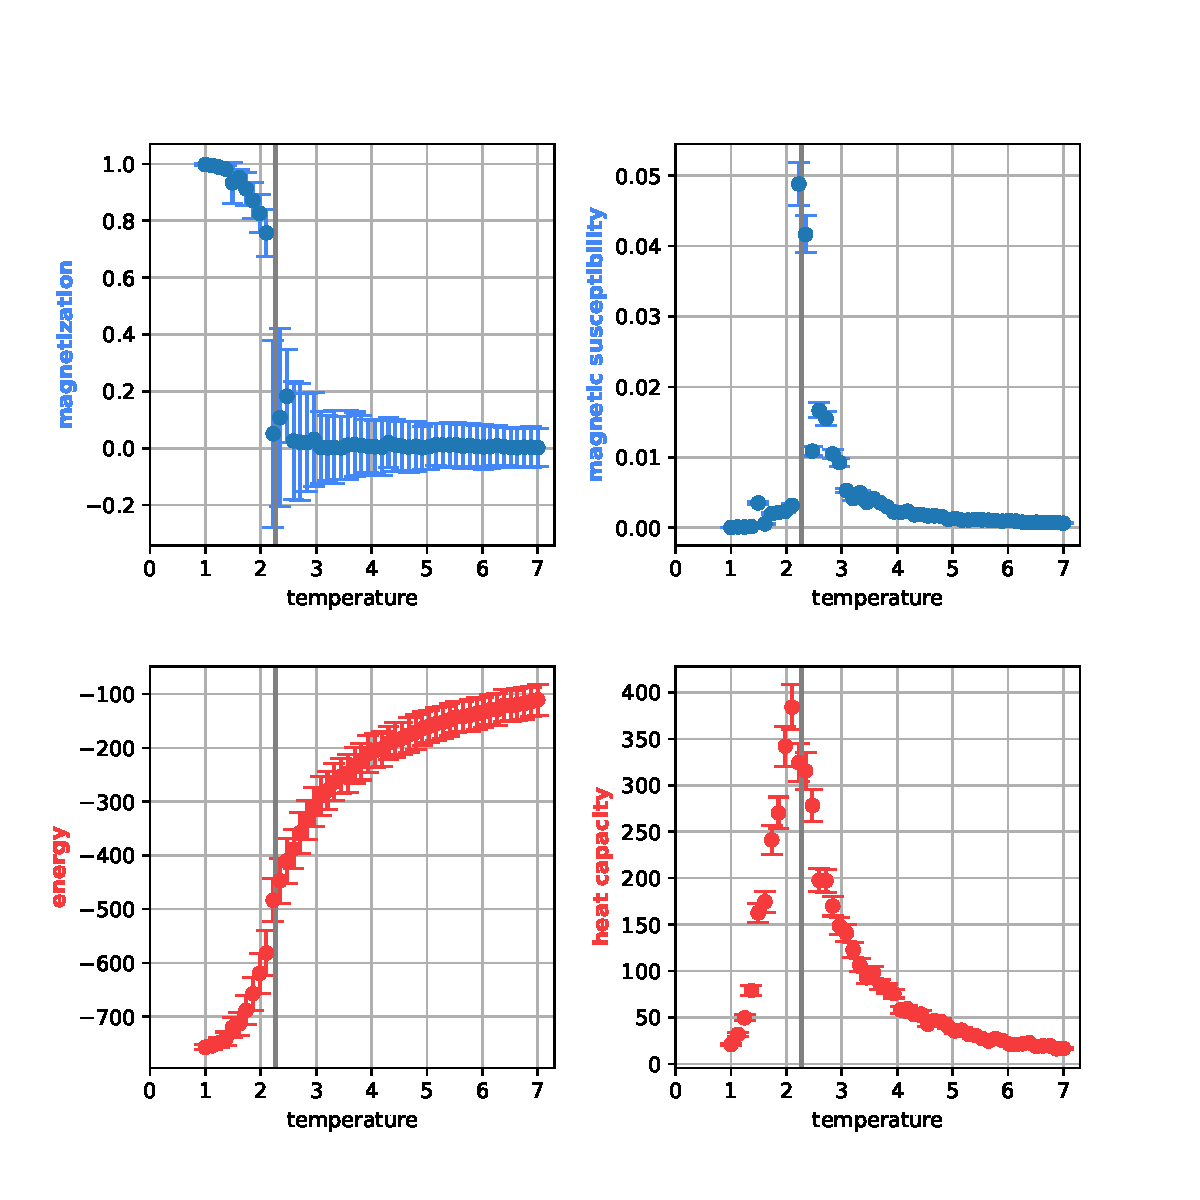
\includegraphics[width=\linewidth]{latex_source/images/ising/2d_scaling.pdf}
    \caption{Dependence of thermodynamic quantities on temperature. The vertical grey line marks the theoretical critical temperature as given by Onsager's formula [Eq: \ref{eq:onsager}]. One can see that the peaks of $C$ and $\Chi$ are very close to the theoretical temperature. For $500$ equilibration steps and $500$ sweep steps at each temperature, the code took $12$ minutes to execute.}
    \label{fig:2d_scaling}
\end{figure}
}